\begin{ZhChapter}

\chapter{若標題太長，則可以分成兩行排列的形式撰寫}

\section{名詞定義（小標）}

定義定義定義定義定義定義\cite{latex2e}，定義定義定義定義，定義定義定義定義定義定義定義定義定義定義，定義定義。

\begin{table*}[htbp]
    \centering
    \caption{表格範例標題} \label{tab: complexity}
    \makebox[\linewidth][c]{
    \renewcommand\arraystretch{1.2}{
        \begin{tabular}{| l | c  c  c  c |}
        \hline
        Protocol & $P$ & $CS_1$ & $CS_2$ & $RG$ \\
        \hline
        MSSMul & $O(1)$, $O(1)$, N/A & $O(n-t)$, $O(n)$, $O(1)$ & $O(n-t)$, $O(n)$, N/A & $O(1)$, $O(n)$, $O(n)$ \\
        SC & $O(1)$, $O(1)$, N/A & $O(n-t)$, $O(n)$, $O(1)$ & $O(n-t)$, $O(n)$, N/A & $O(1)$, $O(n)$, $O(n)$ \\
        \hline 
        \end {tabular}
    }}
\end {table*}

\section{模型說明（小標）}

說明說明說明說明，說明說明說明說明說明說明說明說明說明說明說明說明，說明說明說明說明說明說明說明說明。

\begin{figure*}[htbp]
    \centering
    \includegraphics[width = 0.5\textwidth]{image.jpeg}
    \caption{Cool train station}
    \label{fig: image}
\end{figure*}

% ===== 以下為轉換演示 =====

\section{VMSH: Hypervisor-agnostic Guest Overlays for VMs}

\subsection{System Architecture}

As an independent host process, vmsh runs alongside the hypervisor on the same host machine. vmsh does not modify the hypervisor's source code, nor does it rely on any management API provided by the hypervisor. Instead, vmsh completes all operations externally through ptrace and the underlying KVM API. Figure~\ref{fig:vmsh-arch} presents the system architecture of vmsh (adapted from \cite{Thalheim2022} Figure 2), whose workflow can be divided into the following four steps:

\begin{figure*}[htbp]
    \centering
    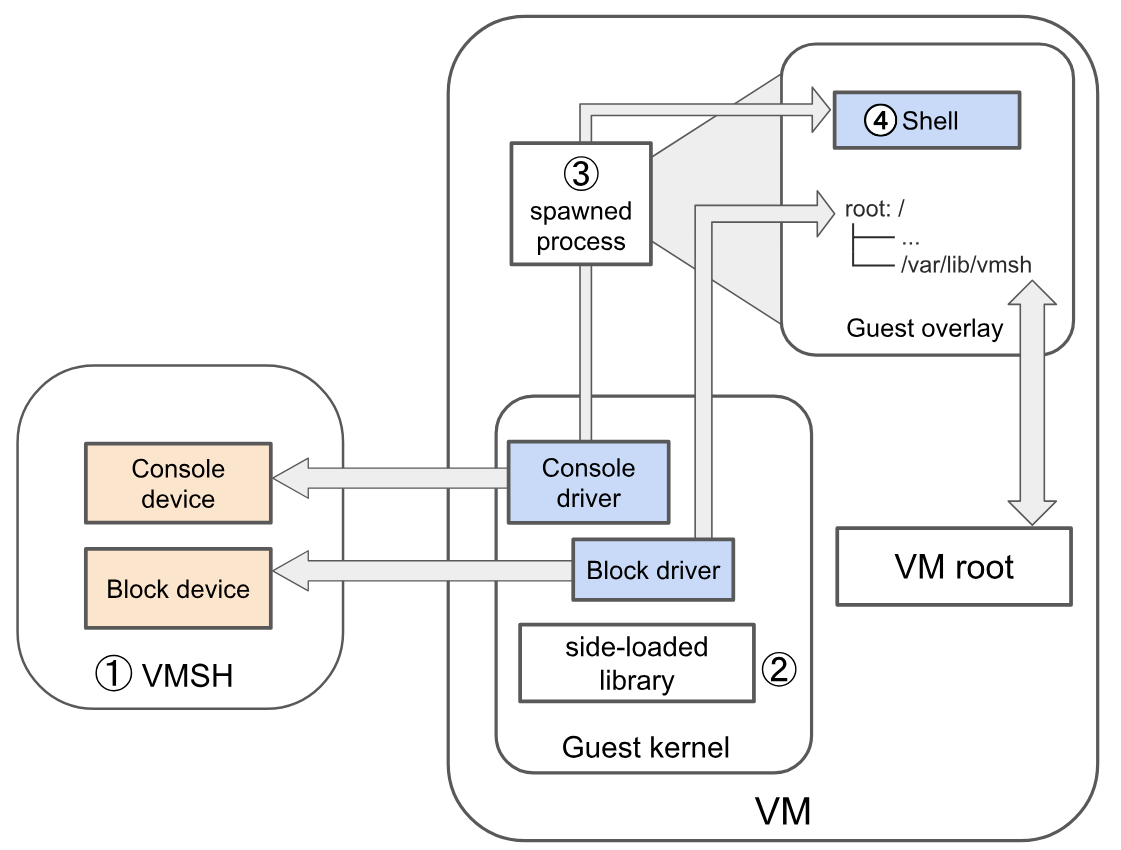
\includegraphics[width=0.8\textwidth]{figures/vmsh-arch.png}
    \caption{System architecture of vmsh. vmsh establishes devices in the guest through side-loading a kernel library. The block device supports the overlay root file system, and the console device handles the I/O of the spawned process. Numbers 1--4 correspond to the four-step workflow. (Adapted from \cite{Thalheim2022})}
    \label{fig:vmsh-arch}
\end{figure*}

% ===== 演示結束 =====

\end{ZhChapter}